\subsection*{Problem 1}
Let $G = (V, E)$ be a simple, connected graph with adjacency matrix $A$
\begin{enumerate}[\indent (a)]
    \item Prove that, for any positive integer $k$, the $(i, j)$-th entry of $A^k$ equals the number of walks of length $k$ from vertex $i$ to vertex $j$ in $G$.
    \item Use this property to show that the number of walks of length 2 starting and ending at vertex $i$ is equal to the degree of $i$.
    \item Determine the graph $G$ if every entry of the matrix $A + A^2$ is equal.
\end{enumerate}


\begin{proof}
Suppose $G = (V, E)$ is a simple, connected graph with adjacency matrix $A$.
\\
\textbf{a)} Note that for vertices $i$ and $j$, since the $(i, j)$-th entry of $A$ corresponds to the number of edges between $i$ and $j$, it equivalently represents the number of walks of length 1 (an edge) that exists between $i$ and $j$. Additionally, we observe that \[ (A^k)_{ij}=\sum_{v_1,v_2,\dots,v_{k-1} \in V} A_{iv_1} A_{v_1v_2} A_{v_2v_3} \cdots A_{v_{k-1}j} \] for any positive integer $k$ where $i,v_1,\dots,v_{k-1},j \in V$ are a sequence of vertices. Because we sum over all intermediary vertices $v_1,v_2,\dots,v_{k-1} \in V$, the $(i, j)$-th entry of $A^k$ corresponds to the number of ways to get from vertex $i$ to vertex $j$ through vertices $v_1,v_2,\dots,v_{k-1}$, which is exactly the number of walks of length $k$ from vertex $i$ to vertex $j$ in $G$.
\\
\textbf{b)} The number of walks of length 2 starting and ending at vertex $i$ is equivalent to $(A^2)_{ii}$. Then, observe that \[ (A^2)_{ii}=A_{i1}A_{1i}+A_{i2}A_{2i}+\dots+A_{in}A_{ni}=\sum_{j=1}^n A_{ij} A_{ji} \]
Note that each term $A_{ij}A_{ji}$ equals $1$ only when $i$ and $j$ are adjacent, and $0$ otherwise. The summed quantity thus accumulates the number of edges that are connected to vertex $i$, which is exactly the degree of $i$.
\\
\textbf{c)}
Observe that $(A+A^2)_{ij}$ counts the number of walks of length 1 or 2 that exist between vertices $i$ and $j$. Since all entries are constant, then the number of walks that are either length 1 or 2 between any two vertices are the same. Note that since the diagonal entries of $A$ are all 0 and the diagonal entires of $A+A^2$ are equal, then the diagonal entries of $A^2$ must equal the non-diagonal entries of $A+A^2$. Thus, the number of paths of length 2 from any vertex $i$ back to itself must be equal to the number of paths of length 1 or 2 between any two distinct vertices. This is only possible if every pair of distinct vertices is adjacent. Thus, the graph must be complete. Note that the trivial solution $A = 0_{n \times n}$ also satisifies the condition. Therfore, the graph $G$ must be either a set of vertices with no edges such that $G=(V,\emptyset)$, or the complete graph $G=K_n$.
\end{proof}

\subsection*{Problem 2}
Prove that the edge set of a graph $G = (V, E)$ can be partitioned into two spanning
trees if and only if $G$ can be constructed from a single vertex using the following two operations:
\begin{enumerate}[\indent (i)]
    \item adding a new vertex $v$ together with two edges connecting $v$ to existing vertices,
    \item subdividing an existing edge $uw$ by introducing a new vertex $v$, replacing $uw$ with $uv$ and $vw$, and connecting $v$ to an existing vertex with an additional edge.
\end{enumerate}

\begin{proof}
We will prove both directions.
\\
($\implies$) Assume $G$ is constructed from the two operations. We need to show it can be partitioned into 2 spanning trees. We will proceed by induction. For the base case, assume $G$ has no edges yet. Here, it can be partitioned into 2 spanning trees, each spanning tree consisting of 0 edges. Now, assume $G$ can be partitioned into 2 spanning trees $T_1$ and $T_2$. If we apply operation 1, we add a vertex $v$ to $G$ connected by two seperate edges $e_1$ and $e_2$. $T_1$ and $T_2$ can recieve $e_1$ and $e_2$ respectively and $T_1$ and $T_2$ remain trees. Thus, $G$ remains being able to be partitioned into 2 spanning trees. If instead we apply operation 2, then we consider some edge $uw$, where $uw$ is some edge either in $T_1$ or $T_2$. This edge is then replaced with $uv$ and $vw$, connecting $v$ to an existing vertex with an additional edge. Without loss of generality, suppose $uw$ is a member of $T_2$. The replacement edges $uv$ and $vw$ then will belong to the same tree $T_2$, allowing $u$, $v$, and $w$ to remain connected in $T_2$. The final edge placed to connect the new vertex $v$ with any other vertex will then always return to a connected segment of the other tree, $T_1$, without creating a cycle and thus preserving the partitions. Therefore, any graph $G$ constructed from the two operations can be partitioned into 2 spanning trees.
\\
($\impliedby$) We will reverse the above argument.
\end{proof}

\subsection*{Problem 3}
Consider the following graph. Run Kruskal's algorithm step by step to find its minimum-weight spanning tree. At each step, indicate which edge is added and the current total weight of the partial spanning forest.

\begin{center}
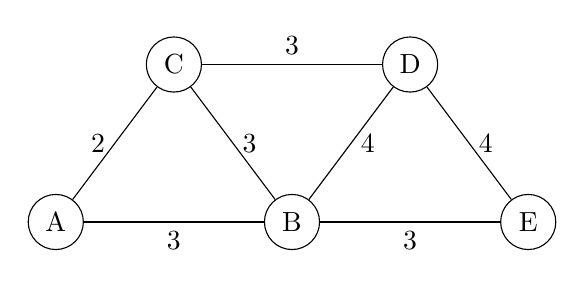
\begin{tikzpicture}[node/.style={circle,draw,minimum size=7mm},>=stealth]
\node[node] (C) at (-0.5,2) {C};
\node[node] (D) at (2.5,2) {D};
\node[node] (A) at (-2,0) {A};
\node[node] (B) at (1,0) {B};
\node[node] (E) at (4,0) {E};
\draw (C) -- (D) node[midway,above] {3};
\draw (A) -- (C) node[midway,left] {2};
\draw (C) -- (B) node[midway,right] {3};
\draw (B) -- (D) node[midway,right] {4};
\draw (D) -- (E) node[midway,right] {4};
\draw (A) -- (B) node[midway,below] {3};
\draw (B) -- (E) node[midway,below] {3};
\end{tikzpicture}
\end{center}

\begin{solution}

\begin{enumerate}[Step 1:]
    \item Add minimum edge $AC$ with cost 2. Current total cost = 2.
    \item Add next minimum edge $CB$ with cost 3. Current total cost = 5.
    \item Add next minimum edge $CD$ with cost 3. Current total cost = 8.
    \item Add next minimum edge $BE$ with cost 3. Current total cost = 11.
\end{enumerate}
All vertices are now connected and we have avoided cycles. The following is our spanning tree:
\begin{center}
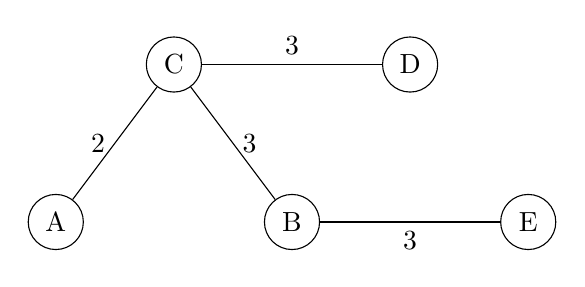
\begin{tikzpicture}[node/.style={circle,draw,minimum size=7mm},>=stealth]
\node[node] (C) at (-0.5,2) {C};
\node[node] (D) at (2.5,2) {D};
\node[node] (A) at (-2,0) {A};
\node[node] (B) at (1,0) {B};
\node[node] (E) at (4,0) {E};
\draw (C) -- (D) node[midway,above] {3};
\draw (A) -- (C) node[midway,left] {2};
\draw (C) -- (B) node[midway,right] {3};
\draw (B) -- (E) node[midway,below] {3};
\end{tikzpicture}
\end{center}

\end{solution}

\subsection*{Problem 4}
Let $G = (V, E)$ be a connected graph with distinct edge weights. Prove that the minimum-weight spanning tree of $G$ is unique

\begin{proof}
Assume for the sake of contradiction that we have two minimum-weight spanning trees of $G$, $A$ and $B$, where $A \ne B$. Without loss of generality, this implies that there exists a set of edges $E = A \setminus B$ with $E \ne \emptyset$. We will then apply the exchange theorem. Let $e \in E$ to be the edge has minimum weight. If we add $e$ to $B$, then we will have formed a cycle. Additionally, there is at least one edge $f$ in this cycle such that $f \in B \setminus A$. Note that since all edge weights of the graph $G$ are distinct, all the edges in this cycle are strictly greater than the weight of the edge $e$, and thus, the weight of $f$ is strictly greater than the weight of $e$. Remove $f$ from this newly constructed $B$ yields a spanning tree $B'$. Note that the total weight of $B' < B$, which implies that $B$ is not minimal, a contradiction. Therefore, $A = B$ and the minimum-weight spanning tree of $G$ is unique.
\end{proof}

\subsection*{Problem 5}
Suppose we stop Kruskal's algorithm as soon as we have selected $k-1$ edges, where $k$ is a fixed integer between $1$ and $|V|$. Show that the resulting forest is optimal in the sense that it minimizes the total weight among all spanning forests with $k$ connected components. 

\begin{proof}
TODO
\end{proof}

\subsection*{Problem 6}
Prove that every connected graph admits a closed walk that uses each edge exactly twice.

\begin{proof}
Let $G$ be a connected graph. Construct a new graph $G'$ by duplicating and doubling every edge in $G$. Then every vertex of $G'$ has even degree, and $G'$ is connected. Since every vertex has an even degree, we know that $G$ has a Eulerian tour, which is a closed walk that traverses each edge in $G'$ exactly once. Since each edge in $G$ appears twice in $G'$, this walk corresponds to a closed walk in $G$ that traverses each edge in $G$ exactly twice.

\end{proof}

\subsection*{Problem 7}
Let $G$ be a graph in which the degree of every vertex is 4. (A graph with all degrees equal to $k$ is called $k\text{-}regular$, so G is a 4-regular graph.) Prove that we can color all edges of $G$ with one of the two colors red and blue, such that every vertex becomes incident to exactly two red and two blue edges.

\begin{proof}
Since every vertex has degree $4$, all vertices have even degree, and thus there exists a Eulerian tour through every edge. Consider a starting vertex $v$ and begin a Eulerian tour through the graph, coloring each red and blue alternating between the two. Now every vertex has 2 colored incident edges, 1 red and 1 blue. If we ignore or remove all these edges from the graph, we are left with a graph where each vertex has degree 2. Note that here, every vertex still has an even degree, and thus, there exists another Eulerian tour through every edge. If we begin another Eulerian tour, coloring each visited red and blue alternating between them, we will have colored all edges, and thus, we are left with a graph where every vertex becomes incident to exactly two red and two blue edges.
\end{proof}

\subsection*{Problem 8}
Let $G$ be a graph in which every vertex has even degree. Show that it is possible to label the edges of $G$ with the integers $1,\dots,m$ (where $m = |E(G)|$) so that, for every vertex, the greatest common divisor of the labels on its incident edges is 1.

\begin{proof}
Since $G$ is a graph in which every vertex has even degree, there exists a Eulerian path. Choose an arbitrary starting vertex $v$ and begin a Eulerian tour through every edge. For the first edge, label it 1. Then label the next edge 2, and continue this pattern. That is, for each subsequent edge, label it with an integer that is 1 greater than the previous edge. Observe that through this process, we have labeled the edges of $G$ with the integers $1,\dots,m$ where $m = |E(G)|$. Additionally, note that for every edge, there exists an edge with some integer $p$ and another integer $p+1$. The greatest common divisor of the labels is therefore $1$, since for any $p \in \mathbb{Z}_{>0}$, $\gcd(p, p+1)=1$.
\end{proof}